\documentclass[12pt]{article} 
\usepackage{longtable}
\usepackage{makecell}
\usepackage{float}
\usepackage{graphicx}
\usepackage{bm}
\usepackage{placeins}
\usepackage{booktabs}
\usepackage{gensymb}
\usepackage{subcaption}
\usepackage{amssymb}
\usepackage{indentfirst}
\usepackage{threeparttable} 
\usepackage{multirow}
\usepackage{tabularx}
\usepackage{aligned-overset}
\usepackage[slantfont,boldfont]{xeCJK}
\usepackage{fontspec}
\renewcommand{\arraystretch}{1.5}
% \usepackage[paperwidth=21cm,paperheight=29.7cm]{geometry}
\usepackage[a4paper,margin=2cm]{geometry}
\setCJKmainfont{SimSun}
\setmainfont{SimSun}
\setsansfont{SimSun}
% 设置正文字体为四号（12pt）
% \renewcommand{\CJKmainfont}{SimSun}
\renewcommand{\CJKfamilydefault}{\CJKrmdefault}
\renewcommand{\normalsize}{\fontsize{12pt}{18pt}\selectfont}
\normalsize

\title{光学自组实验实验报告}
\author{2411545 邱凯锐}
\date{2025.12.5}

\begin{document}
\maketitle
\section{双波罗棱镜望远镜}
\subsection{实验原理}
\subsubsection{望远镜}

Figure 1 是开普勒式望远镜调焦于无限远时的光路图。物镜将无限远处的物体在其焦平面上成一倒立实象，然后由目镜将此实象放大，使之在无限远处，供人眼观察。
由 Figure 1 可知，望远镜的视角放大率为

\begin{equation}
    \Gamma=\frac{tg\omega_i}{tg\omega_e}=\frac{tg\omega'}{tg\omega}=\frac{y'/f'_e}{-y'/f_o'}=-\frac{f_e'}{f_o'}
\end{equation}

\begin{figure}[H]
    \centering
    
\includegraphics[width=0.6\textwidth]{fig1.png}
    \caption{调焦于无限远的开普勒望远镜}
\end{figure}

在许多情况下，用望远镜所观察的物体并非处于无限远，这时通过改变物镜和目镜之间距离进行调焦，使物体通过物镜所成的实象位于目镜的物方焦平面以
里，再经目镜在明视距离外成一虚象。其光路如 Figure 2
所示。这时被观察物体对眼睛的视角为
\begin{equation}
    tg \omega_e=tg\omega=\frac{y_1}{S_1+S_2+S_3}
\end{equation}
通过望远镜后视角为
\begin{equation}
    tg \omega_i=tg\omega'=\frac{y_2}{S_3}
\end{equation}
又 $y_2/y_1=S_2/S_1$ ，所以望远镜在观察有限远物体时的视角放大率为

\begin{equation}
    \Gamma=\frac{tg\omega_i}{tg\omega_e}=\frac{S_2(S_1+S_2+S_3)}{S_1S_3}
\end{equation}

\begin{figure}[H]
    \centering
    
\includegraphics[width=0.6\textwidth]{fig4.png}
    \caption{观察有限远物体时的望远镜光路}
\end{figure}

\subsubsection{波罗棱镜}
保罗棱镜是由玻璃块塑造成的等腰直角三棱镜，末端平面对着直角。
\begin{figure}[H]
    \centering
    
\includegraphics[width=0.4\textwidth]{fig3.png}
    \caption{波罗棱镜}
\end{figure}

\subsection{实验过程}
实验仪器：光源和物、物镜、目镜、波罗棱镜两个。

按照光路图摆放器件，并调节各器件位置，直至观察带清晰的像。

\begin{figure}[H]
    \centering
    \begin{subfigure}[b]{0.4\textwidth}
        \centering
        
\includegraphics[width=\textwidth]{fig2.png}
        \caption{双波罗棱镜望远镜光路}
    \end{subfigure}
    \hfil
    \begin{subfigure}[b]{0.4\textwidth}
        \centering
        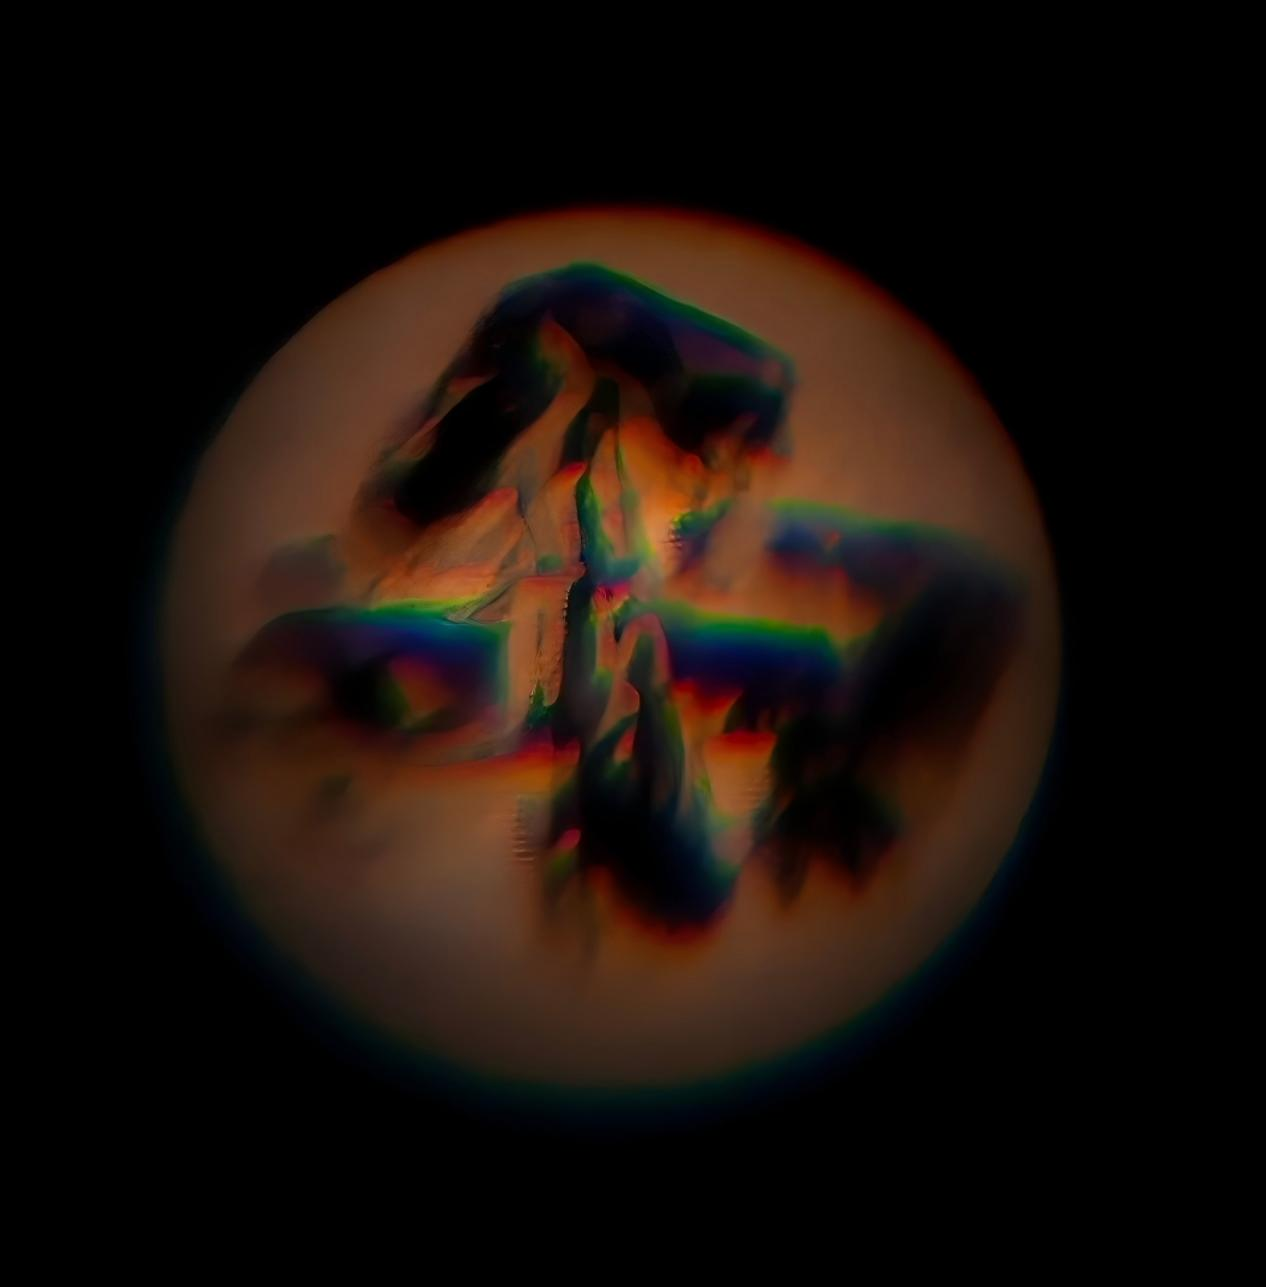
\includegraphics[width=\textwidth]{fig1.jpg}
        \caption{望远镜成象结果}
    \end{subfigure}
    \caption{双波罗棱镜望远镜}
\end{figure}

\section{光栅光谱仪}
\begin{figure}[H]
    \centering
    
\includegraphics[width=0.5\textwidth]{fig5.png}
    \caption{光栅光谱仪光路图}
\end{figure}

按照光路图摆放器件，逐一调整各元器件位置和角度，使得光屏上出现对应谱线。

\begin{figure}[H]
    \centering
    \begin{subfigure}[b]{0.4\textwidth}
        \centering
        
\includegraphics[width=\textwidth]{fig7.jpg}
        \caption{光栅光谱仪实验装置}
    \end{subfigure}
    \hfil
    \begin{subfigure}[b]{0.4\textwidth}
        \centering
        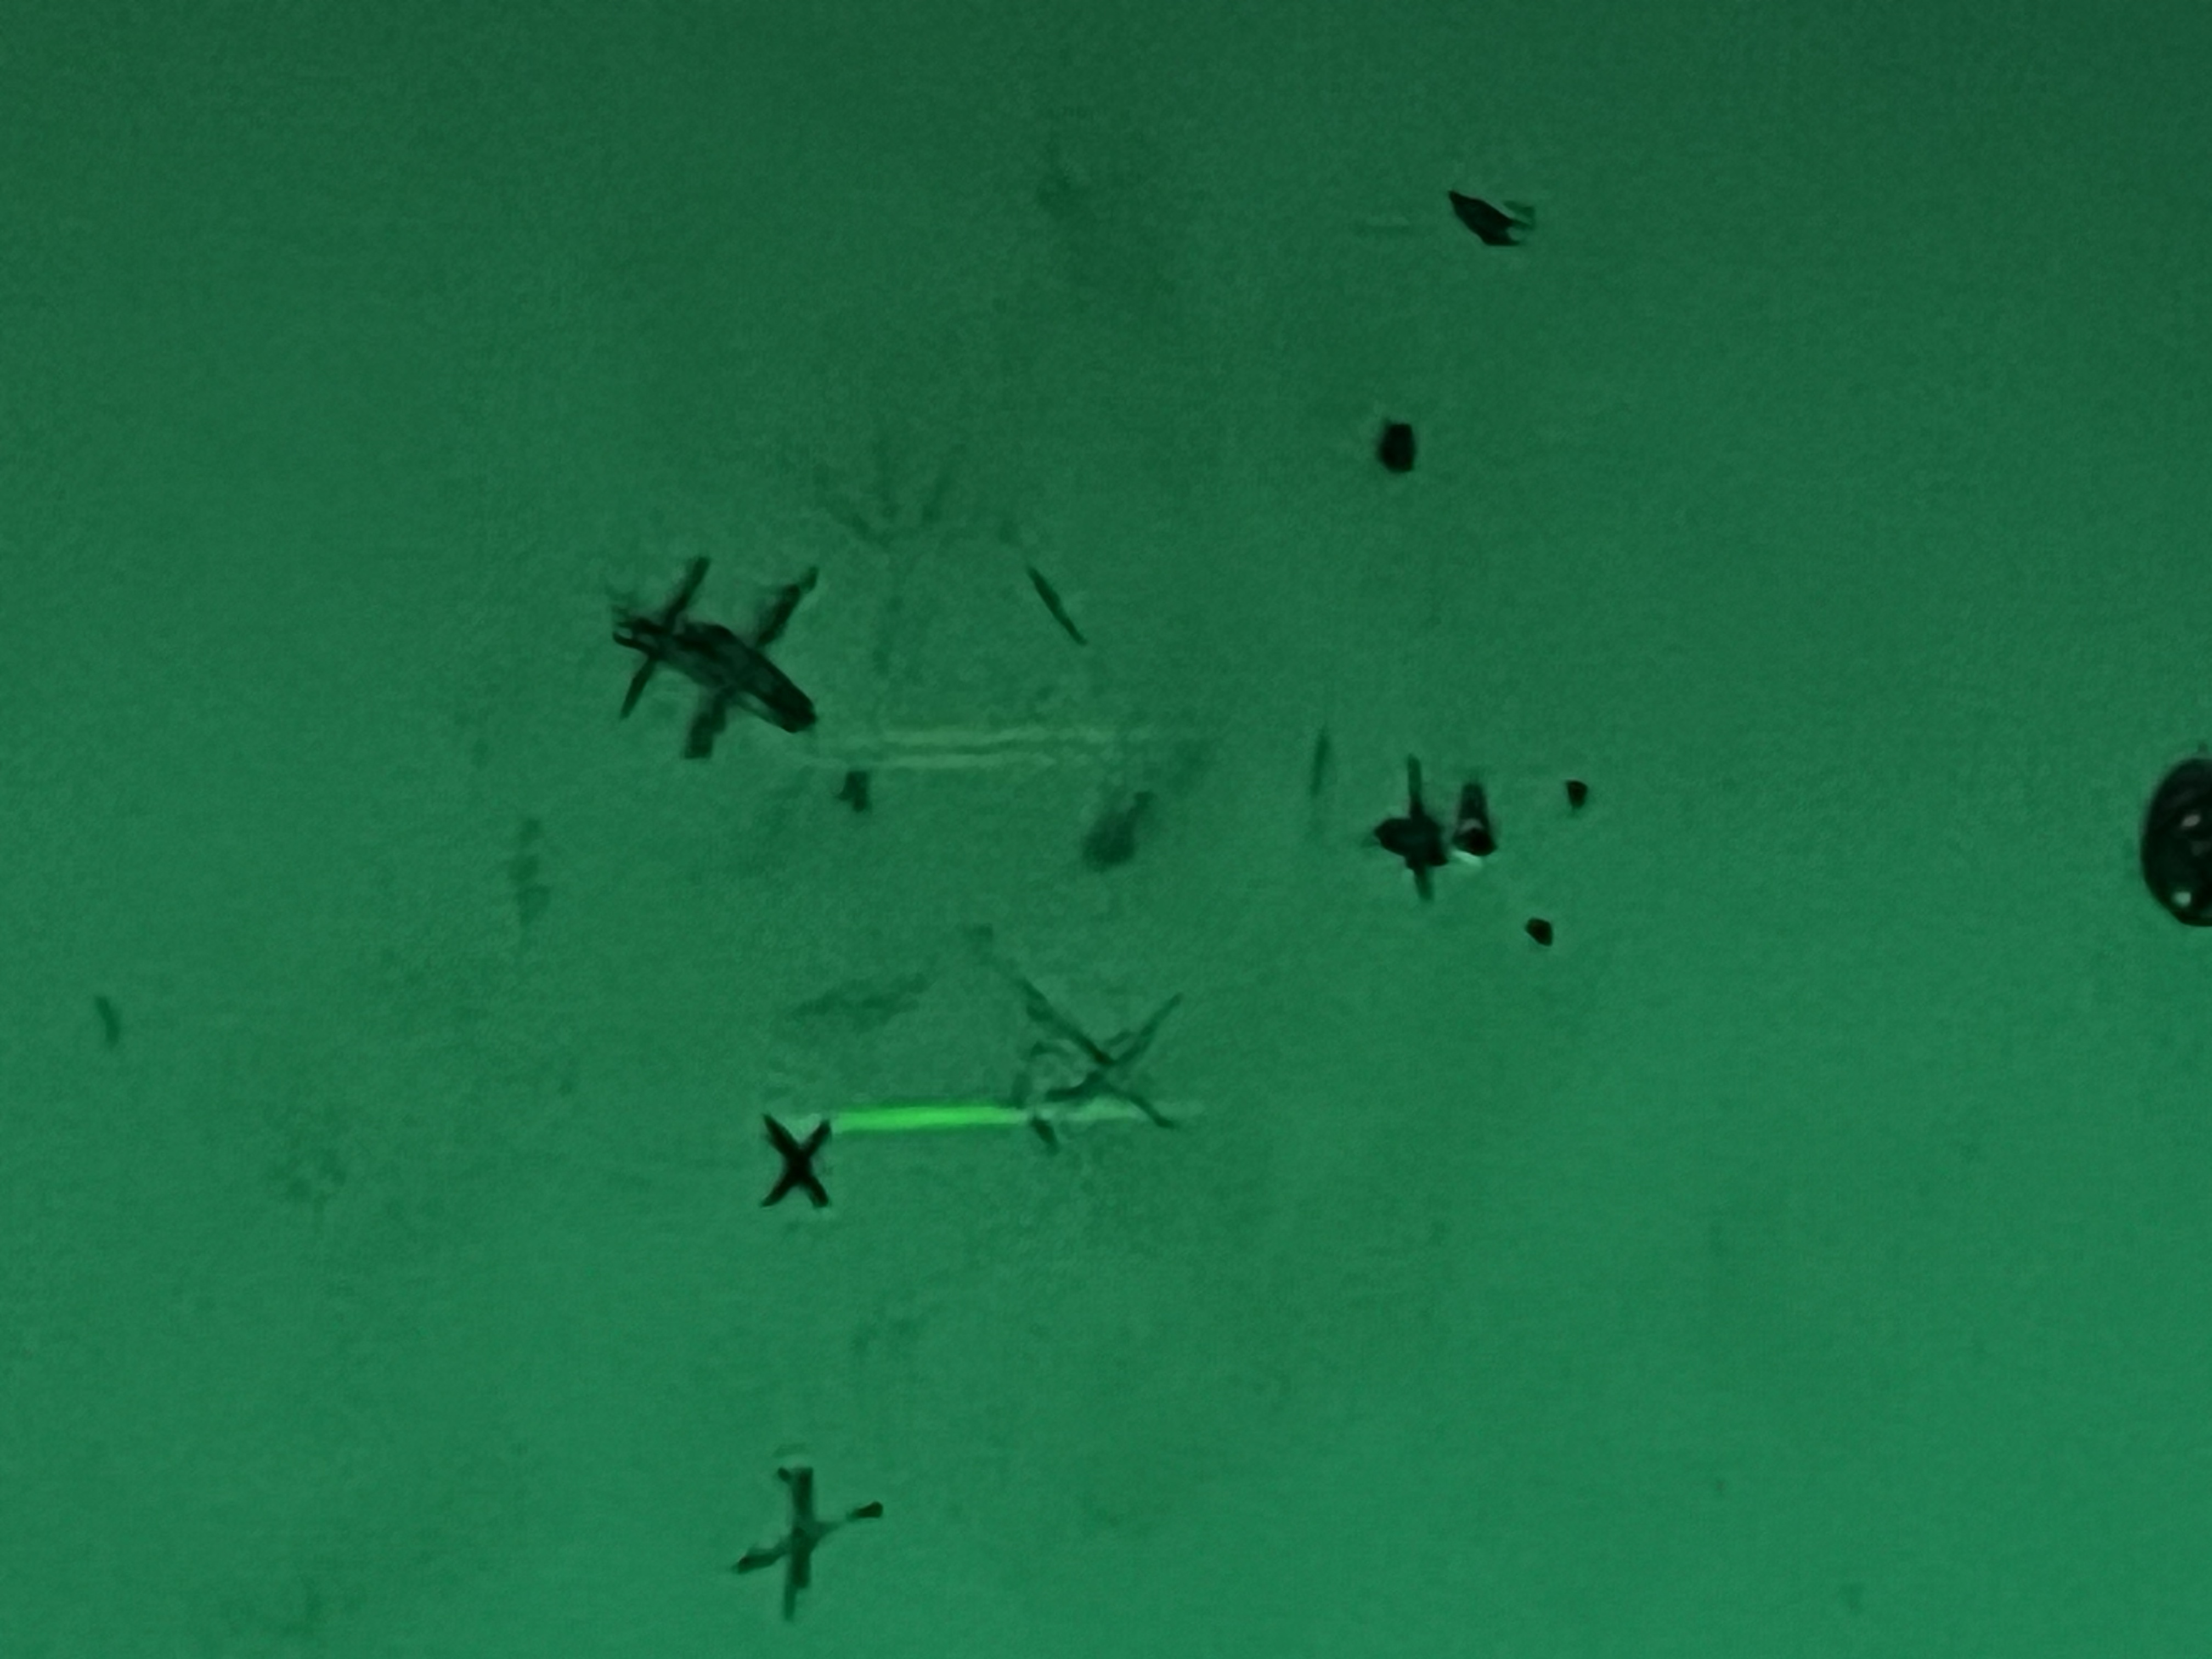
\includegraphics[width=\textwidth]{fig8.jpg}
        \caption{谱线}
    \end{subfigure}
    \hfil
    \begin{subfigure}[b]{0.4\textwidth}
        \centering
        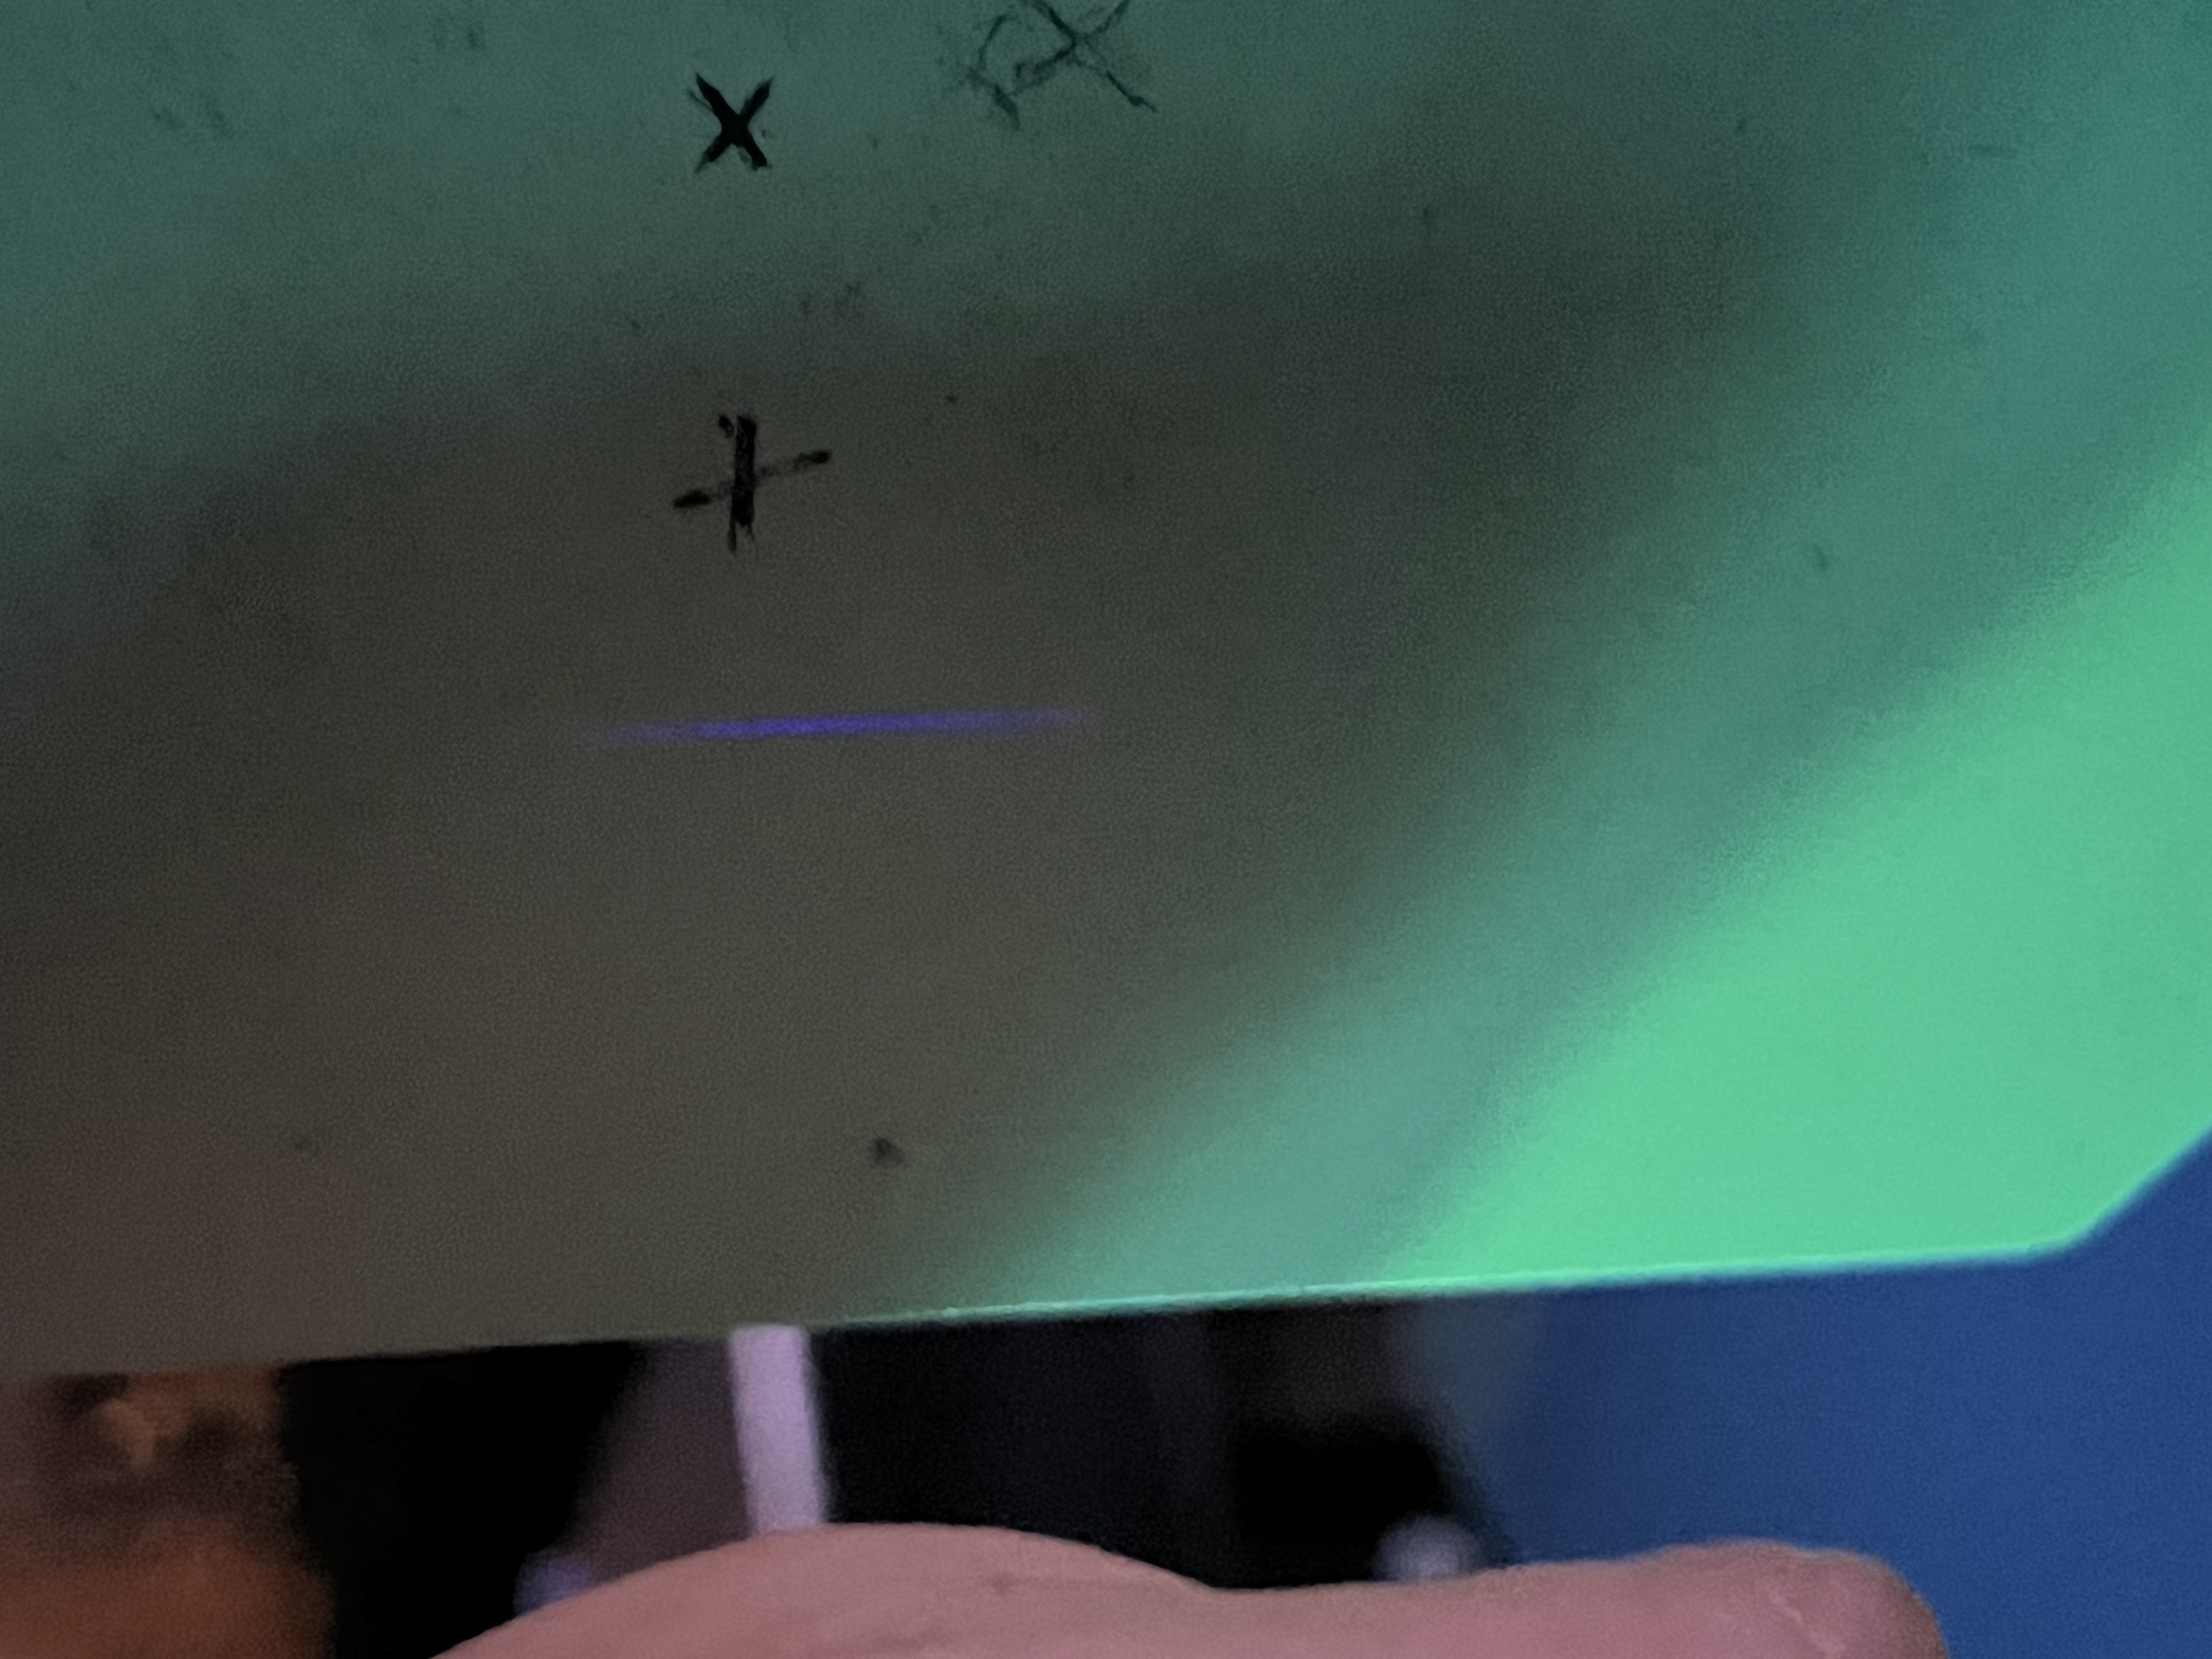
\includegraphics[width=\textwidth]{fig9.jpg}
        \caption{谱线}
    \end{subfigure}
    \hfil

    \caption{光栅光谱仪实验过程}
\end{figure}




\end{document}
